\documentclass[10pt,a4paper]{article}
\usepackage[latin1]{inputenc}
\usepackage{amsmath}
\usepackage{amsfonts}
\usepackage{amssymb}
\usepackage{graphicx}
\usepackage{hyperref}
\usepackage{glossaries}
\usepackage{float}

\newcommand{\kx}{k_x}
\newcommand{\ky}{k_y}
\newcommand{\meff}{m_\text{eff}}

\newcommand{\img}{./images}
\loadglsentries{glossary.tex}
\makeglossaries
\begin{document}
\title{Progress}
\maketitle
%%%%%%%%%%%%%%%%%%%%%%%%%%%%%%%%%%%%%%%%%%%%%%%%%%%%%%%%%%%%%%%%%%%%%%%%%%%%%%%
\section{System description}
	\begin{figure}[H]
		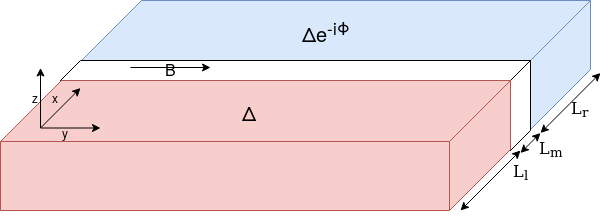
\includegraphics[width=\linewidth]{\img/system.png}
		\caption{System overview}
	\end{figure}
	
	\begin{align}
		H &= H_0(\tau_z \otimes \sigma_0) + 
		H_\text{Z} (\tau_0 \otimes \sigma_z) +
		(\tau_z \otimes H_\text{SO}) +
	 H_\text{SC}(\tau_y \otimes \sigma_0) \\
		H_0 &= \frac{\hbar^2}{2\meff}\left(\kx^2 + \ky^2\right) - \mu \\
		H_\text{Z} &= g \mu_B B  \left(\Theta(-x) - \Theta(L_m-x)\right)  \\
		H_\text{SO} &= \alpha \left( \ky \sigma_x - \kx \sigma_y \right)\\
		H_\text{SC} &= \Delta \exp \left(i \theta \Theta(x-L_m) \right)
	\end{align}

	Where: 
	\begin{equation}
	\Theta(x) = 
	\begin{cases}
	1,& x>0\\
	0,& \text{otherwise}
	\end{cases}
	\end{equation}

	\subsection{System parameters}
	\begin{table}
		\begin{tabular}{|c|c|c|c|}
			\hline 
			Variable & Description & Typical value & Default value \\ 
			\hline 
			$g_\text{factor}$ & Magnetic g-factor of material & ~10 & 10 \\ 
			\hline 
			$\mu$ & Chemical potential &  10 - 30 meV & 1 meV\\ 
			\hline 
			$\alpha$ & Spin orbit coupling strength &  30 meV nm & 30 meV nm \\ 
			\hline 
			$\Delta$ & Superconducting gap & 0.2 - 0.3 meV & 0.18 meV\\ 
			\hline 
			$B$ & In-plane magnetic field strength along stripe direction(y) & 0 - 1 T & 0.2 T \\ 
			\hline 
			$\phi$ & Relative phase between superconductors &  0 - 2$\pi$ & $\pi$\\ 
			\hline 
			$\text{L}_\text{l}$ & Width of left superconductor & $\infty$ & 500 nm \\
			\hline 
			$\text{L}_\text{m}$ & Width of right superconductor & $\infty$ & 500 nm \\
			\hline
			$\text{L}_\text{r}$ & Width of middle "normal" strip & 100 - 1000 nm & 250 nm \\
			\hline
			$\text{L}_\text{y}$ & Height of system & \textgreater1000 nm & 4000 nm\\
			\hline
		\end{tabular} 
	\caption{Description of system parameters, along with typical valuses, as well as a default value which is the used value when no other value has been specified.}
	\label{tbl:system_pars}
	\end{table}
%%%%%%%%%%%%%%%%%%%%%%%%%%%%%%%%%%%%%%%%%%%%%%%%%%%%%%%%%%%%%%%%%%%%%%%%%%%%%%%
\section{Topological overview of the system}
%------------------%
	\subsection{important metrics}
		\begin{itemize}
			\item \Gls{Ethouless}
				\begin{align}\label{eq:thouless}
				E_\text{Th} = TN\delta
				, && \delta = \frac{\hbar^2 \pi^2}
				{2 m_e \left( 2 L_m \right)^2}
				\end{align}
			Where $T$ is the transparancy of the junction, and N the number of bands.
			\item Pfaffian sign
			\item Topological energy gap
			\item (critical) current, phase offset in current-phase relationship
		\end{itemize}
%------------------%
	\subsection{Varying magnetic field strength and superconducting phase}
		From the Pientka paper, we would expect an image plot of whether the system is topological or not, with axes superconducting phase and magnetic field, to form diamond structures repeating along the magnetic field axis, spaced apart with a distance equal to the Thouless energy.
		
		We indeed find this to be the case(figure \ref{fig:lmZPpfaf}). We however find that beyond a certain magnetic field strength the bands cross, and the model becomes unphysical.
	%------------------%
	\subsection{Varying system dimensions}
	Widening the junction lowers the Thouless energy, which makes the topological regime accesible at lower magnetic fields, but at the same moment lowering the energy gap.
	\begin{table}[H]
		\centering
		\begin{tabular}{|c|c|}
			\hline 
			$L_\text{m} (nm)$ & $E_\text{Th} (meV)$ \\ 
			\hline 
			250 & 1.05 \\ 
			\hline 
			500 & 0.523 \\ 
			\hline 
			1000 & .262 \\ 
			\hline 
			5000 & .0523 \\ 
			\hline 
		\end{tabular} 
		\caption{Thouless energy for different system widths calculated using \ref{eq:thouless}, asssuming unit transparency.}
		\label{table:thouless}
	\end{table}
	
	\begin{figure}[H]
		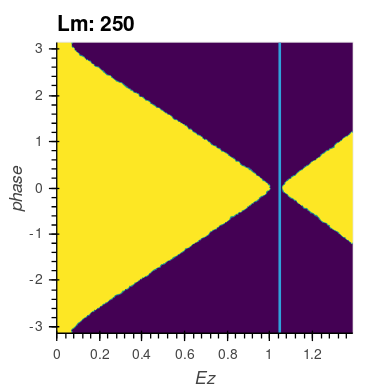
\includegraphics[width=0.5\textwidth]{\img/lmZPpfaf/pB250.png}
		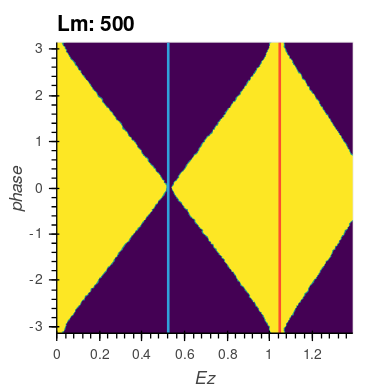
\includegraphics[width=0.5\textwidth]{\img/lmZPpfaf/pB500.png}
		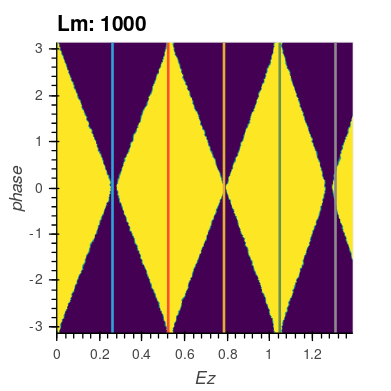
\includegraphics[width=0.5\textwidth]{\img/lmZPpfaf/pB1000.png}
		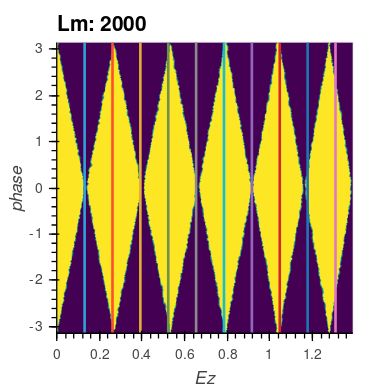
\includegraphics[width=0.5\textwidth]{\img/lmZPpfaf/pB2000.png}
		\caption{Topological regime(blue is topological) vs superconducting phase and magnetic field strength, for different strip widths. The lines indicate integer multiples of the Thouless energy, see table \ref{table:thouless}}
		\label{fig:lmZPpfaf}
	\end{figure}
	
	\begin{figure}[H]
		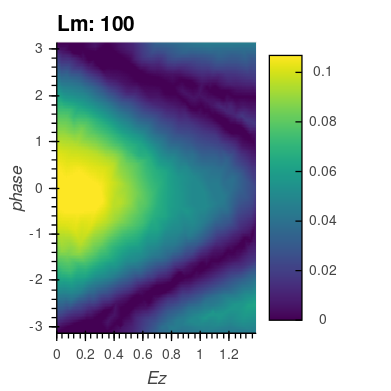
\includegraphics[width=0.5\textwidth]{\img/lmgap/lm100.png}
		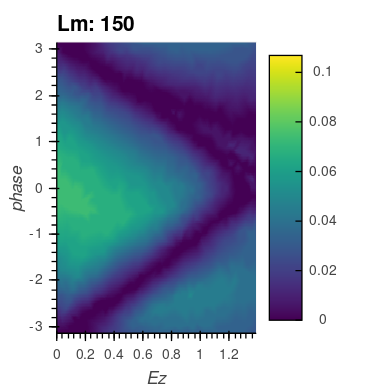
\includegraphics[width=0.5\textwidth]{\img/lmgap/lm150.png}
		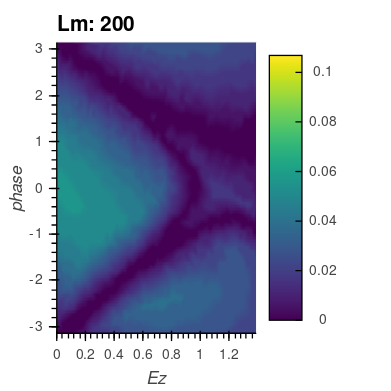
\includegraphics[width=0.5\textwidth]{\img/lmgap/lm200.png}
		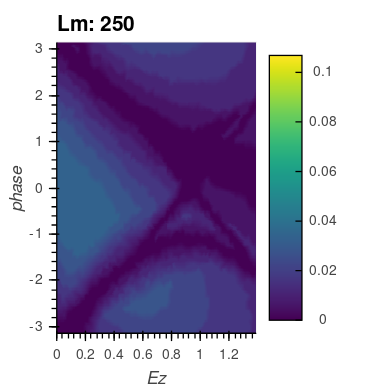
\includegraphics[width=0.5\textwidth]{\img/lmgap/lm250.png}
		%				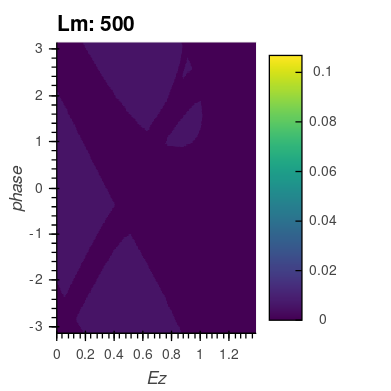
\includegraphics[width=0.24\textwidth]{\img/lmgap/lm500.png}
		\caption{Topological regime(blue is topological) vs superconducting phase and magnetic field strength, for different strip widths. The lines indicate integer multiples of the Thouless energy, see table \ref{table:thouless}}
		\label{fig:lmZPcurr}
	\end{figure}
%------------------%		
	\subsection{Varying chemical potential and magnetic field strength}
		From the Pientka paper, we would expect 
			\begin{figure}[H]
				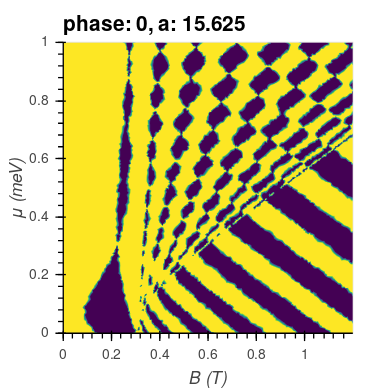
\includegraphics[width=0.3\textwidth]{muB0.png}
				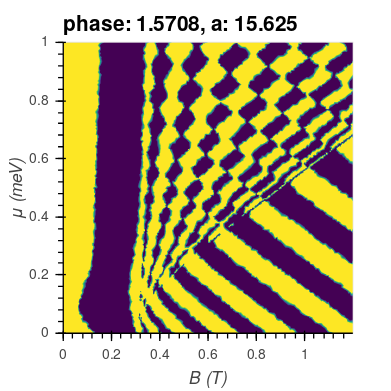
\includegraphics[width=0.3\textwidth]{muB5.png}
				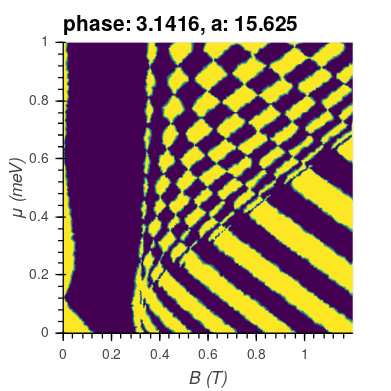
\includegraphics[width=0.3\textwidth]{muB1.png}
				\caption{Topological regime(blue is topological) vs chemical potential and magnetic field strength, assuming zeeman field in the superconductor}
			\end{figure}
%------------------%	
	\subsection{Varying spin-orbit}
		\begin{figure}[H]
			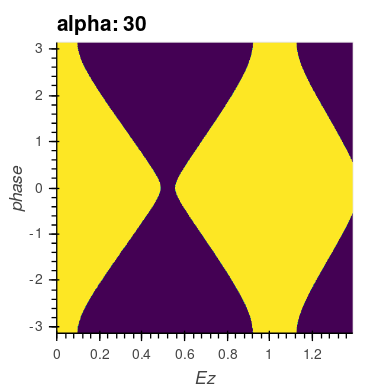
\includegraphics[width=0.192\textwidth]{\img/spinorbitZP/a30.png}
			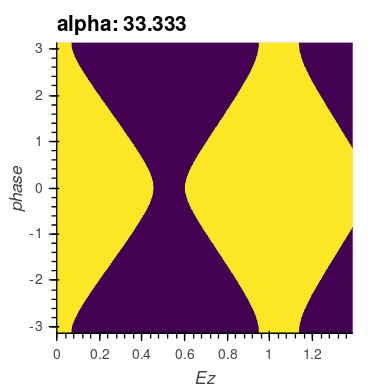
\includegraphics[width=0.192\textwidth]{\img/spinorbitZP/a33.png}
			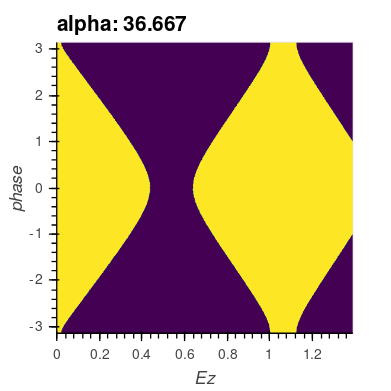
\includegraphics[width=0.192\textwidth]{\img/spinorbitZP/a36.png}
			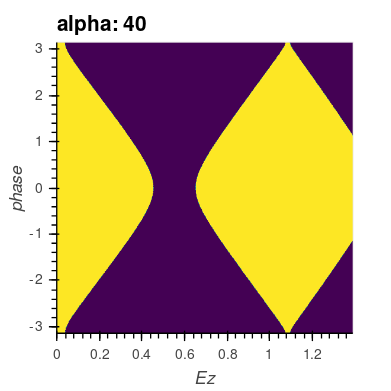
\includegraphics[width=0.192\textwidth]{\img/spinorbitZP/a40.png}
			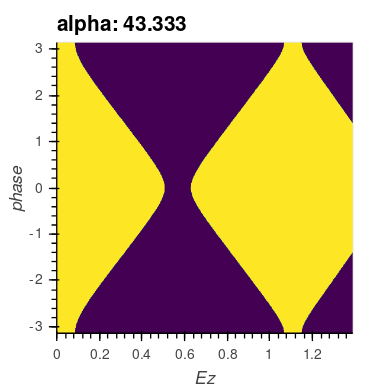
\includegraphics[width=0.192\textwidth]{\img/spinorbitZP/a43.png}
			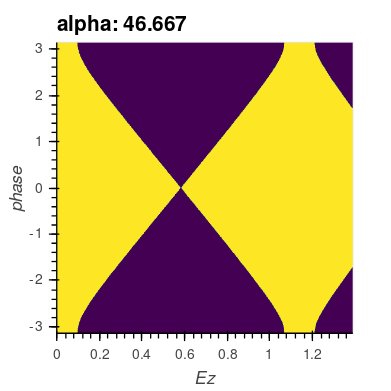
\includegraphics[width=0.192\textwidth]{\img/spinorbitZP/a46.png}
			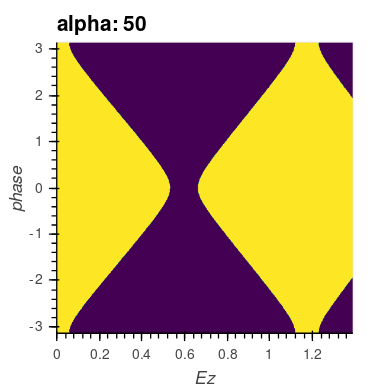
\includegraphics[width=0.192\textwidth]{\img/spinorbitZP/a50.png}
			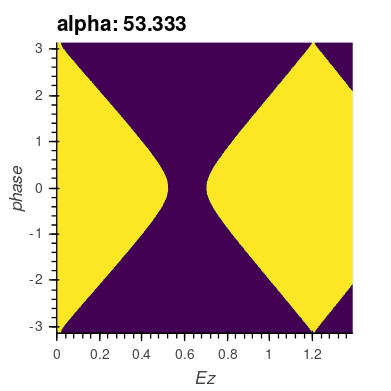
\includegraphics[width=0.192\textwidth]{\img/spinorbitZP/a53.png}
			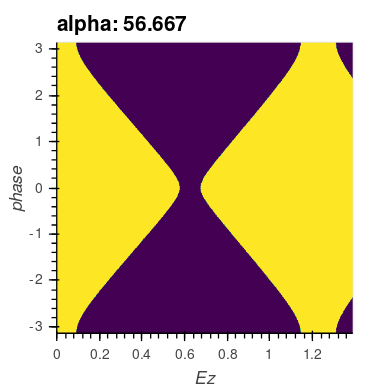
\includegraphics[width=0.192\textwidth]{\img/spinorbitZP/a56.png}
			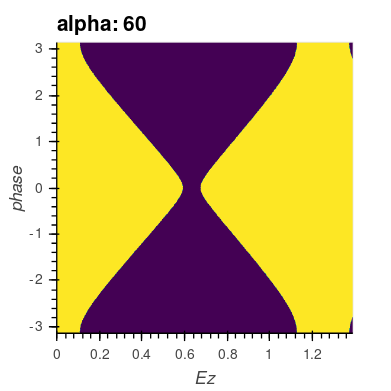
\includegraphics[width=0.192\textwidth]{\img/spinorbitZP/a60.png}
			\caption{Phase zeeman plot with increasing spin orbit}
		\end{figure}
%------------------%	
	\subsection{Varying superconducting gap}
		\begin{figure}[H]
			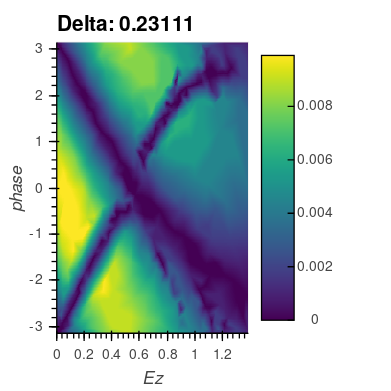
\includegraphics[width=0.24\textwidth]{\img/deltagapZPcurrent/d02.png}
			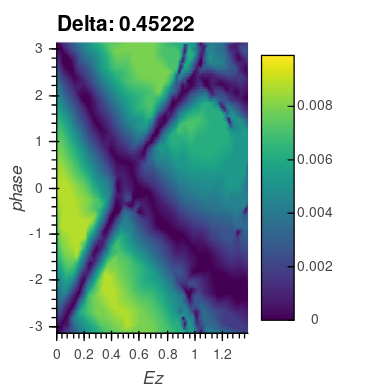
\includegraphics[width=0.24\textwidth]{\img/deltagapZPcurrent/d045.png}
			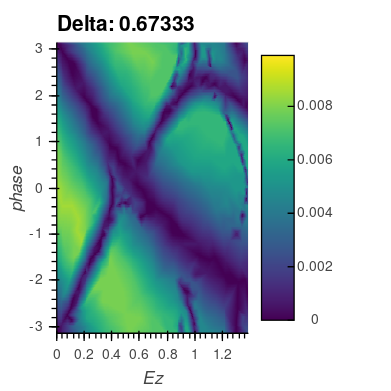
\includegraphics[width=0.24\textwidth]{\img/deltagapZPcurrent/d067.png}
			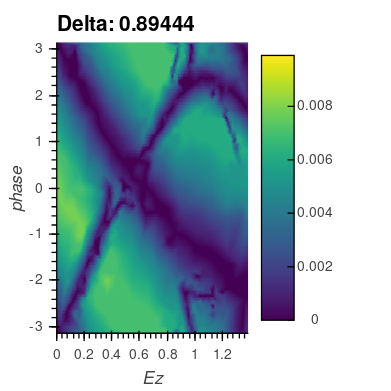
\includegraphics[width=0.24\textwidth]{\img/deltagapZPcurrent/d089.png}
			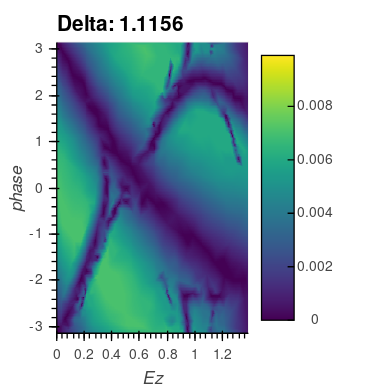
\includegraphics[width=0.24\textwidth]{\img/deltagapZPcurrent/d11.png}
			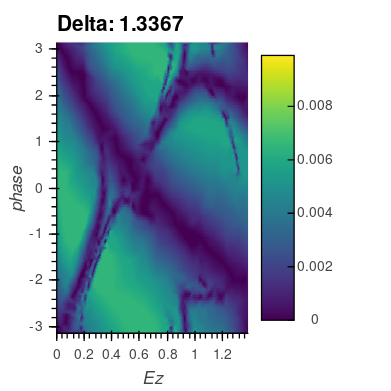
\includegraphics[width=0.24\textwidth]{\img/deltagapZPcurrent/d133.png}
			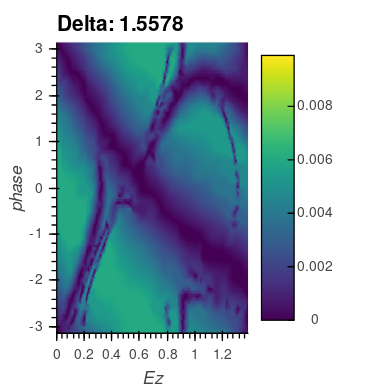
\includegraphics[width=0.24\textwidth]{\img/deltagapZPcurrent/d155.png}
			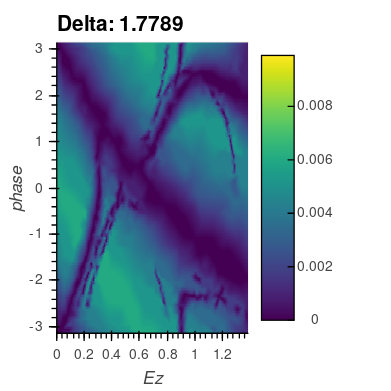
\includegraphics[width=0.24\textwidth]{\img/deltagapZPcurrent/d178.png}
			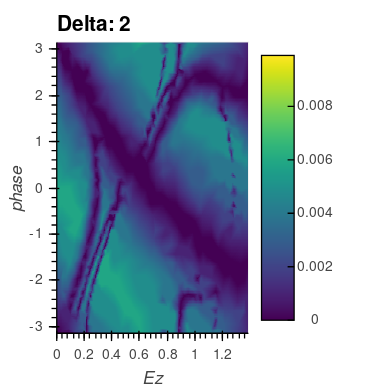
\includegraphics[width=0.24\textwidth]{\img/deltagapZPcurrent/d200.png}
			\caption{Phase zeeman plot with increasing spin orbit}
		\end{figure}

%%%%%%%%%%%%%%%%%%%%%%%%%%%%%%%%%%%%%%%%%%%%%%%%%%%%%%%%%%%%%%%%%%%%%%%%%%%%%%%
\clearpage
\printglossaries
\end{document}

